\documentclass[a4paper, 8pt]{article}
\usepackage[latin1]{inputenc}
\usepackage[T1]{fontenc}
\usepackage[francais]{babel}
\usepackage{entete}
\usepackage{noitemsep}
\usepackage{euscript} 
\usepackage{amsmath,amssymb,amsfonts,amsthm}
\usepackage{graphicx,graphics,epsfig,subfigure,color}
\usepackage{url}
%\usepackage{algorithm2e}
\usepackage{multicol}
\usepackage{a4wide}
\usepackage{latexsym}
\usepackage{verbatim}
% \setlength{\textheight}{23.5cm}
% \setlength{\topmargin}{-1cm}
% \setlength{\textwidth}{155mm}
% \setlength{\oddsidemargin}{2mm}

\usepackage[paper=a4paper, bmargin=1.5cm, tmargin=1.5cm, lmargin=1.5cm, rmargin=1.5cm]{geometry} 
%\renewcommand{\baselinestretch}{0.85}

%\input{macroAlgo}
%\dontprintsemicolon

\setlength{\parindent}{0pt}  %%suppression indentation


\begin{document}
\selectlanguage{francais}
\author{D. Fourer}
\newcommand{\universityname}{IUT d'\'Evry Val d'Essonne}
\newcommand{\deptname}{D\'epartement TC (S3)}
\newcommand{\years}{2023-2024}

%------------------- TITRE -----------------------------------------
\date{Septembre 2023} 
\TDHead{\universityname}{\deptname}{R3.12 RCN3, \years}{\large TD5: site internet avec Wordpress (bases)}
%\TDHead{DUT TC}{}{\large TIC3: Fonctions avanc\'ees d'un tableur}
%-------------------------------------------------------------------
%
%\underline{Objectifs:} Ma\^itrise du content management system (CMS) WordPress
%\vspace{-0.5cm}
%\section{} %%duree 30min, 1h maxi
%
Wordpress est un Syst\`eme de Gestion de Contenu (SGC) ou Content Management System (CMS)
libre d\'evelopp\'e en PHP/mysql permettant de cr\'eer rapidement un site internet 
sans connaissance avanc\'ee en programmation.

 \exost Connectez-vous sur \verb?https://iut2.fourer.fr/<nom_7caracteres>_<prenom_3caracteres>?
\begin{enumerate}
 \item Choisissez la langue puis configurez votre site en renseignant un \underline{identifiant}, un \underline{mot de passe} et votre \underline{adresse email}. Cliquez sur ``install wordpress'' apr\`es avoir v\'erifi\'e les information saisies. %(\textbf{attention, il ne sera plus possible de revenir en arri\`ere en cas d'erreur}).
 \item Vous recevrez alors un courriel contenant les informations de votre site puis vous arriverez sur votre tableau de bord. \textbf{Ce site internet sera strictement personnel et servira uniquement pour les TPs.}
 \end{enumerate}
%\vspace{-0.3cm}
\begin{figure}[!ht]
\begin{center}
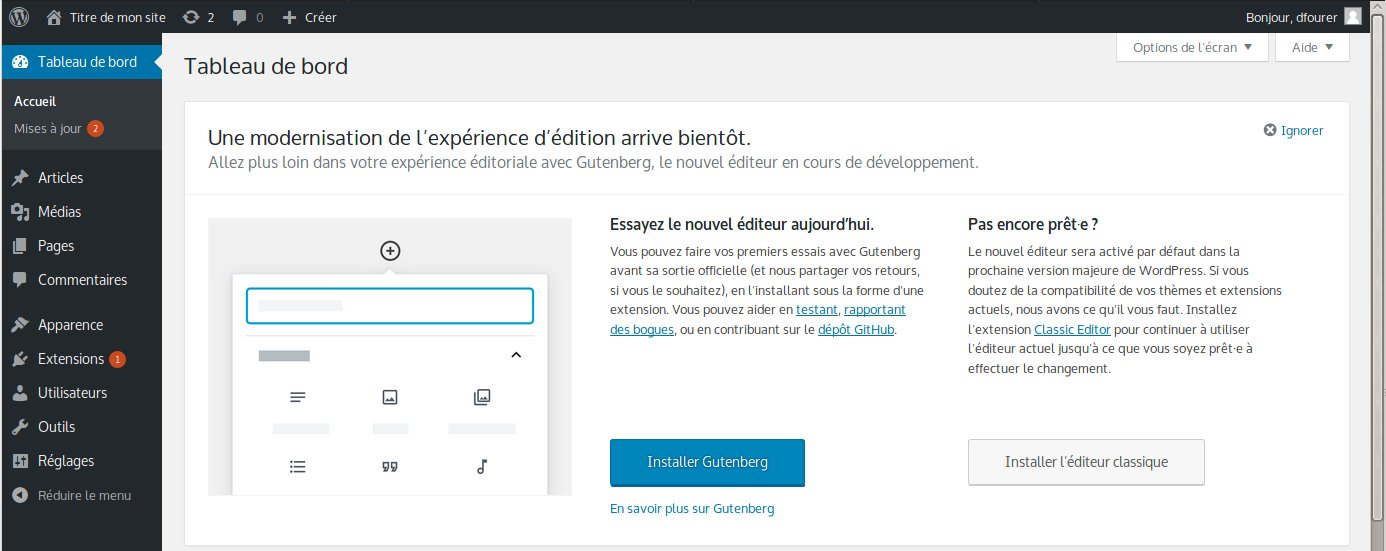
\includegraphics[height=6cm]{tableau_de_bord.jpg} %width=0.7\textwidth, 
\end{center}
\caption{Tableau bord. Accessible via: $https://<$adresse\_du\_site$>$\textbf{/wp-admin} .} % /wp_admin %%\verb?<adresse_du_site>/wp-admin?
\end{figure} % $>\\$\textbf{/wp_admin}
%\vspace{-0.4cm}
%% Version sur wordpress.com
%% chargement d'un fichier audio et creation d'un script.
% \exost Connectez-vous sur \url{http://www.wordpress.com} puis cliquez sur \textbf{Get Started}.
% \begin{enumerate}
%  \item Renseignez les champs \textbf{email}, \textbf{login} et \textbf{password}.
%  \item Remplissez le formulaire (optionnel) et cliquez sur \textbf{continue}.
%  \item Choisissez un nom puis s\'electionnez l'adresse propos\'ee gratuitement (\textbf{free}).
%  \item Apr\`es la derni\`ere \'etape, consultez vos mails et cliquez sur le lien de validation.
% \end{enumerate}
% %
% \textit{Attention, notez bien l'adresse propos\'ee par wordpress:} \textbf{\quad\quad\quad\quad\quad~~~~~~~~~~~~~~~~~~~~~~~~.wordpress.com} \\
% Cette adresse est strictement personnelle et vous permettra d'acc\'eder \`a votre site.
%\section{Param\'etrage du site}

\exost \textbf{Configurez l'apparence de votre site internet:} Vous pourrez consulter le r\'esultat des modifications \textbf{enregistr\'ees} en ouvrant la version publique de votre site
sur une seconde fen\^etre de votre navigateur (pensez \`a l'actualiser r\'eguli\`erement avec la touche ``F5'').
\begin{enumerate}
 \item Installez un nouveau \textbf{th\`eme} (``Twenty Sixteen'') puis personnalisez le (``Apparence/personnaliser'' et ``R\'eglages/General'').
 \item D\'esactivez les \textbf{widgets} inutiles de sorte \`a conserver uniquement la fonction de recherche ainsi que les articles et commentaires r\'ecents. 
 %Ajoutez le widget ``calendrier'' dans la barre (vous pouvez d\'eplacer les widgets en les faisant glisser avec le clic gauche).
 \item Ajoutez un \textbf{widget} ``texte'' de contact en bas de page. Ajoutez-y des informations de contact que vous souhaitez afficher \`a vos visiteurs (e.g. mail, tel, etc.).
\end{enumerate}

%% creation de pages / Articles
\exost Les \underline{articles} d\'eveloppent en profondeur un sujet (class\'e dans une cat\'egorie) et permettent aux visiteurs de poster des commentaires pour l'enrichir.\\
Les \underline{pages} servent \`a structurer votre site et \`a afficher des informations statiques \`a vos visiteurs.\\
Les \underline{permaliens} permettent un acc\`es direct \`a un article ou une page de votre site.
%
\begin{enumerate}
 \item Cr\'eez une \textbf{cat\'egorie} (``Articles/Cat\'egories'') ``Mes activit\'es'' pour laquelle vous choisirez le \textit{slug} ``activities''.
 \item Ajouter un \textbf{article} dans la \textbf{cat\'egorie} ``Mes activit\'es'', intitul\'e ``IUT'' dans lequel vous donnerez une br\^eve description de la formation que vous suivez (e.g. liste et contenu des cours suivis, nom des enseignants, etc.). 
 Vous pouvez ajouter des \textbf{\'etiquettes} qui vous semblent pertinentes puis cliquez sur ``publier'' quand vous avez termin\'e.
 \item Ajoutez une \textbf{page} ``Qui suis-je?'' dans laquelle vous donnerez une br\`eve description de qui vous \^etes.
\end{enumerate}
Vous pouvez ajouter librement des \textbf{m\'edias} \`a partir de fichiers divers (audio .mp3, video .mp4 ou images .jpg/.gif) qui seront alors disponibles depuis votre \textbf{biblioth\`eque de m\'edias}.

\clearpage
%% Menu
\exost Cr\'eez un nouveau \textbf{menu} (``apparence/menu'') que vous nommerez ``Menu1''. D\'efinissez le comme \textbf{menu principal} puis modifiez sa structure comme suit:
\begin{center}
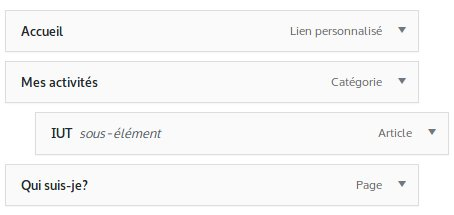
\includegraphics[width=0.3\textwidth]{menu1.jpg} 
\end{center}
\begin{enumerate}
 \item Ajouter un bouton ``accueil'' qui redirigera vers la premi\`ere page de votre site (par d\'efaut, l'article ``Bonjour tout le monde'' que vous pourrez modifier ult\'erieurement).
 \item Ajouter la cat\'egorie ``Mes activit\'es''
 \item Ajouter enfin les pages ``IUT'' comme sous-\'el\'ement de ``Mes activit\'es'' et la page ``Qui suis-je''.
\end{enumerate}
Pensez \`a enregistrer vos modifications pour que ce menu apparaisse dans la barre de titre de votre site. 

%% Extensions

\exost Les extensions permettent d'ajouter des fonctionnalit\'es \`a Wordpress et de d\'evelopper tout son potentiel.
\begin{enumerate}
 \item Dans la rubrique ``Extensions'', recherchez ``WPForms'' que vous \textbf{installerez} puis que vous \textbf{activerez}.
 \item Cr\'eez ensuite un nouveau \textbf{formulaire de contact simple} que vous appellerez ``contact''.
 \item Apr\`es \^etre sorti de l'\'editeur, retournez dans la liste des formulaires (``WpForms/Tous les formulaires'') puis notez le code associ\'e au formulaire contact de la forme: \textbf{[wpforms id="xx"]}.
 \item Ajoutez ensuite ce code \`a la fin de la page ``Qui suis-je?'' pour ajouter un formulaire de contact.
\end{enumerate}




%T\'el\'echargez wordpress sur \url{https://wordpress.org/download/}, d\'ecompressez les fichiers dans le dossier web (www).
%Dans le dossier
% 
% \exost Ouvrez le fichier \verb? classe.xls ? Effectuez un tri des noms des \'etudiant par ordre alphab\'etique (ordre lexicographique croissant)
% en conservant sur chaque ligne l'affectation initiale des notes pour chaque \'etudiant.
% 
% \section{Cr\'eation de contenu} %%duree 30min, 1h maxi
% 
% \exost Choix du style
% 
% \exost Configuration des utilisateurs et des droits d'acc\`es
% 
% 
% 
% \section{Edition des pages} %%duree 30min, 1h maxi
% 
% \exost Modifiez la page d'accueil.
% 
% \exost 





\end{document}

% End Of File

